\documentclass[preprint,proceedings]{rmaa}


%%%
%%% Define any personal macros here
%%% 

% These are some I use in typesetting example code
\newcommand{\bs}{\textbackslash}
\newcommand{\CS}[1]{\texttt{\textbackslash #1}}
% roman subscripts in math
\newcommand{\Sub}[1]{_\mathrm{#1}}
% a command to specify possible linebreak points in an email address 
\newcommand{\D}{\discretionary{}{}{}}

%%%
%%% Article preamble commands (title, authors, abstract, etc.) 
%%% None of these produce any output themselves, they just set things 
%%% up for \maketitle
%%%

% This is only used for making the header for the preprint version
\SetYear{2016}
\SetConfTitle{XV LARIM}

% Please use mixed case here, since this title gets propagated onto
% the web page, ADS entry, etc. 
  \title{Laniakea in a cosmological context}
  
  \author{S. D. Hernandez-Charpak\altaffilmark{1} and
    J. E. Forero-Romero\altaffilmark{1}}  

\altaffiltext{1}{Departamento de F\'isica, Universidad de los Andes,
    Cra 1 18A-10, Bloque Ip, Bogot\'{a}, Colombia.
    (sd.hernandez204\D{}@uniandes\D{}.edu.\D{}co).}



  % List of authors used to construct table of contents
  \listofauthors{S. D. Hernandez-Charpak \& J. E. Forero-Romero}
  % Each author in Surname, Initials format, used in generating Author
  % Index entries.
  \indexauthor{Hernandez-Charpak, S. D.}
  \indexauthor{Forero-Romero, J. E.}


% No \abstract or \resumen for poster papers

% Keywords must be from the standard list and in alphabetical order. 
\addkeyword{H~II regions}
\addkeyword{ISM: Jets and outflows}
\addkeyword{Stars: Pre-main sequence}
\addkeyword{Stars: Mass loss}

%%%
%%% Beginning of document proper
%%%
\begin{document}
% Typeset article header
\maketitle 
%%%Resumen en Español%%%
\boldabstract{A partir de observaciones del flujo c\'{o}smico
local se ha definido nuestro superc\'{u}mulo local, Laniakea. En este trabajo presentamos
un estudio sobre simulaciones de N-cuerpos con el fin de establecer la significancia de
Laniakea en un contexto cosmol\'{o}gico. 
Exploramos diferentes algoritmos para definir superc\'{u}mulos  a partir del campo de
velocidades de la materia oscura en las simulaciones.
Resumimos las propiedades de la poblaci\'{o}n de superc\'{u}mulos por su abundancia a
un volumen total y distribuci\'{o}n de forma. 
Encontramos que superc\'{u}mulos similares en tama\~{n}o y estructura a Laniakea son
poco comunes en un contexto cosmol\'{o}gico amplio.}

%%%Abstract%%%

\boldabstract{Recent observations used local cosmic flow information to
    define our local supercluster, Laniakea. 
    In this work we present a study on large cosmological N-body
    simulations aimed at establishing the significance of Laniakea in a
    cosmological context.
    We explore different algorithms to define superclusters from the dark
    matter velocity field in the simulations. 
    We summarize the properties of the supercluster population by their
    abundance at a given total volume and its shape distribution.
    We find that superclusters similar in size and structure to Laniakea are
    relatively uncommon on a broader cosmological context.}

Tully et al. defined our home supercluster, Laniakea, as the region where the peculiar
velocity flows converge. Laniakea is found to be contained in a 160 Mpc/h diameter
sphere containing a very dense region called the Great Attractor.
We designed a method to find superclusters in dark matter N-body simulations and tested
our method in a simulation of boxsize 250 Mpc/h. We based our method on the analysis of
the eigenvalues $\lambda_1$, $\lambda_2$ and
 $\lambda_3$ of the velocity shear tensor:
\begin{equation}
  \label{eq:mjump}
  \Sigma _{\alpha\beta} = -\frac{1}{2 H_0} \left( \frac{\partial v_{\alpha}}{\partial
  x_{\beta}} + \frac{\partial v_{\beta}}{\partial x_{\alpha}} \right) .
\end{equation}
From these eigenvalues we form two dimensionless quantities: the fractional anisotropy
(FA):
\begin{equation}
  \label{eq:njump}
   FA = \frac{1}{\sqrt{3}} \sqrt{\frac{( \left( \lambda_1 - \lambda_3 \right)^2 +
   \left( \lambda_2 - \lambda_3 \right)^2 + \left( \lambda_1 - \lambda_2 \right)^2 
   )}{\lambda^{2}_1 + \lambda^{2}_2 + \lambda^{2}_3}},
\end{equation}
which tells us if a collapse or expansion is anisotropic (FA=1) or isotropic (FA=0) and the velocity divergence,
normalized by the Hubble constant:
\begin{equation}
  \label{eq:tjump}
  VDH=\lambda_1 + \lambda_2 + \lambda_3 = \frac{- \nabla \cdot \vec{v}}{H_0},
\end{equation}
which tells us if the velocity flows are collapsing (dense region, $VDH>0$).
We are looking for regions dense ($VDH>0$), containing a highly dense locality
($VDH>1.0$), as Laniakea, and bellow a certain threshold of FA.
We use a modified Friends-Of-Friends algorithm, after an CIC interpolation and a finite
elements calculation. We resume our results in
\textbf{Figure
\ref{fig:simple}} and find that: \textbf{Laniakea is atypically larger} than the detected
superclusters and
\textbf{our method is robust} as the largest regions are detected independently of the
FA
thresholds and modifying the grid size in the interpolation do not influence our
results.
\begin{figure}[!t]
  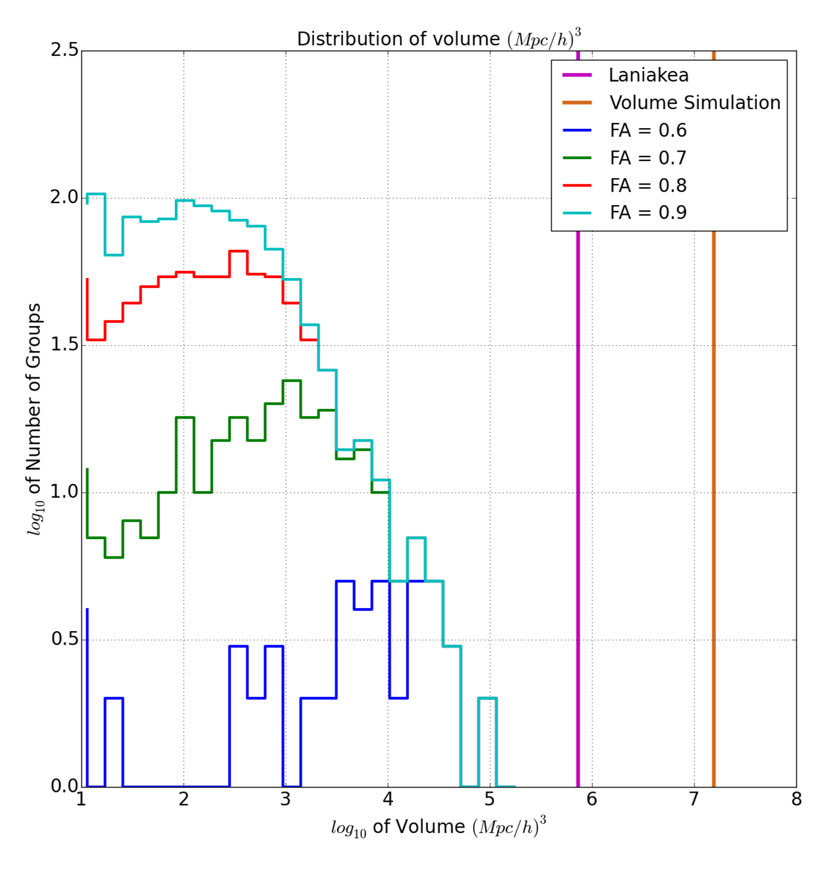
\includegraphics[width=\columnwidth]{SDHernandezSTDivJFig1}
  \caption{Distributions of volumes for different seed FA thresholds.
  %The growth FA is lower than 0.9. The growth VDH is 0.0. The VDH for the seeds is 1.0. We can
%see how Laniakea is larger than the detected structures and smaller than the total
%simulation volume. We can see that as we increase the seeds FA threshold there are
%more regions of small volume detected and that the larger regions detected are always
%detected independently of the seed FA threshold.
}
  \label{fig:simple}
\end{figure}


\begin{thebibliography}

\bibitem{1} R. Brent Tully, Hlne. Courtois, Yehuda Hoffman and Daniel Pomarde. 
{\em The Laniakea Supercluster of galaxies}, Nature, 513 (7516):71-73, September 2014 
 
\bibitem{2} Yehuda Hoffman, Ofer Metuki, Gustavo Yepes, Stefan Gottlöber, Jaime E. Forero-Romero, Noam I. Libeskind and Alexander Knebe. 
{\em A kinematic classification of the cosmic web}, Monthly Notices of the Royal Astronomical Society, 425: 2049–2057, August 2012

\bibitem{3} Noam I. Libeskind, Yehuda Hoffma, Jaime E. Forero-Romero, Stefan Gottlöber, Alexander Knebe, Matthias Steinmetz and Anatoly Klypin. 
{\em The velocity shear tensor: tracer of halo alignment}, Monthly Notices of the Royal Astronomical Societ, 428 (3):2489-2499, January 2013
  
\end{thebibliography}

\end{document}
